\documentclass[journal]{IEEEtran}
\usepackage{enumerate} 
\usepackage[spanish,activeacute]{babel}
\usepackage{graphicx}
\usepackage[latin1]{inputenc}

\hyphenation{op-tical net-works semi-conduc-tor}


\begin{document}
\title{Contador habilitado por bot�n sin rebotes.}
\author{Pedro A. Moreno \\
Departamento de Estudios Multidisciplinarios, Campus Irapuato Salamanca, Universidad de Guanajuato, Yuriria, Guanajuato, M\'exico. \\
Email: pa.morenovazquez@ugto.mx

\thanks{Marzo 21, 2017}}
\markboth{Micrioprocesadores y Microcontroladres,  Marzo~2017}%
{Shell \MakeLowercase{\textit{et al.}}: Bare Demo of IEEEtran.cls for IEEE Journals}



\maketitle

\begin{abstract}

Se us� un microcontrolador PIC16F84A para crear un contador el cual cuente solamente cuando un bot�n es presionado, ademas se elimin� el ruido que el bot�n crea.
 
\end{abstract}

%\begin{IEEEkeywords}
%IEEE, IEEEtran, journal, \LaTeX, paper, template.
%\end{IEEEkeywords}

\IEEEpeerreviewmaketitle

\section{Introducci\'on }

\IEEEPARstart{E}{l} microcontrolador PIC16F84A puede ser usado para crear contadores de manera ascendente los cuales est�n habilitados por una entrada, esta entrada puede ser digital o anal�gica. Si la entrada es anal�gica esta puede causar ruido o se�ales inesperadas, propias de todo elemento anal�gico, que no deben afectar el funcionamiento original del circuito. 

\section{Metodolog\'ia }

\subsubsection{Materiales}
\begin{itemize}
    \item 1 circuito 74LS245.
    \item 1 microcontrolador PIC16F84A.
    \item 1 push button.
    \item 8 LED.
    \item 8 resistencias de 300 $\Omega$.
    \item2 resistencias de 10 $k   {  }\Omega$.
    \item Fuente de alimentaci�n.
\end{itemize}


\subsubsection{Desarrollo}
Primeramente se construy� el circuito, figura 1, para posteriormente crear el c�digo donde se defini� un registro de 8 bits donde se le iba incrementar un valor cuando la entrada registrara un 1. Desafortunadamente el componente f�sico de entrada sufre de vibraciones no deseadas por lo que estas deben ser eliminadas, para esto se ocup� de una rutina de tiempo con duraci�n de 30.3 mili segundos, un tiempo suficiente para que las vibraciones, tambi�n conocidas como rebotes, no afecten la funcionalidad del programa.
Despu�s se implement� un c�digo que impide que el registro aumente sin parar cuando haya un 1 continuo, esto se logr� al esperar por fuerza un cero en la entrada para poder continuar el proceso.


\begin{figure}
  \centering
    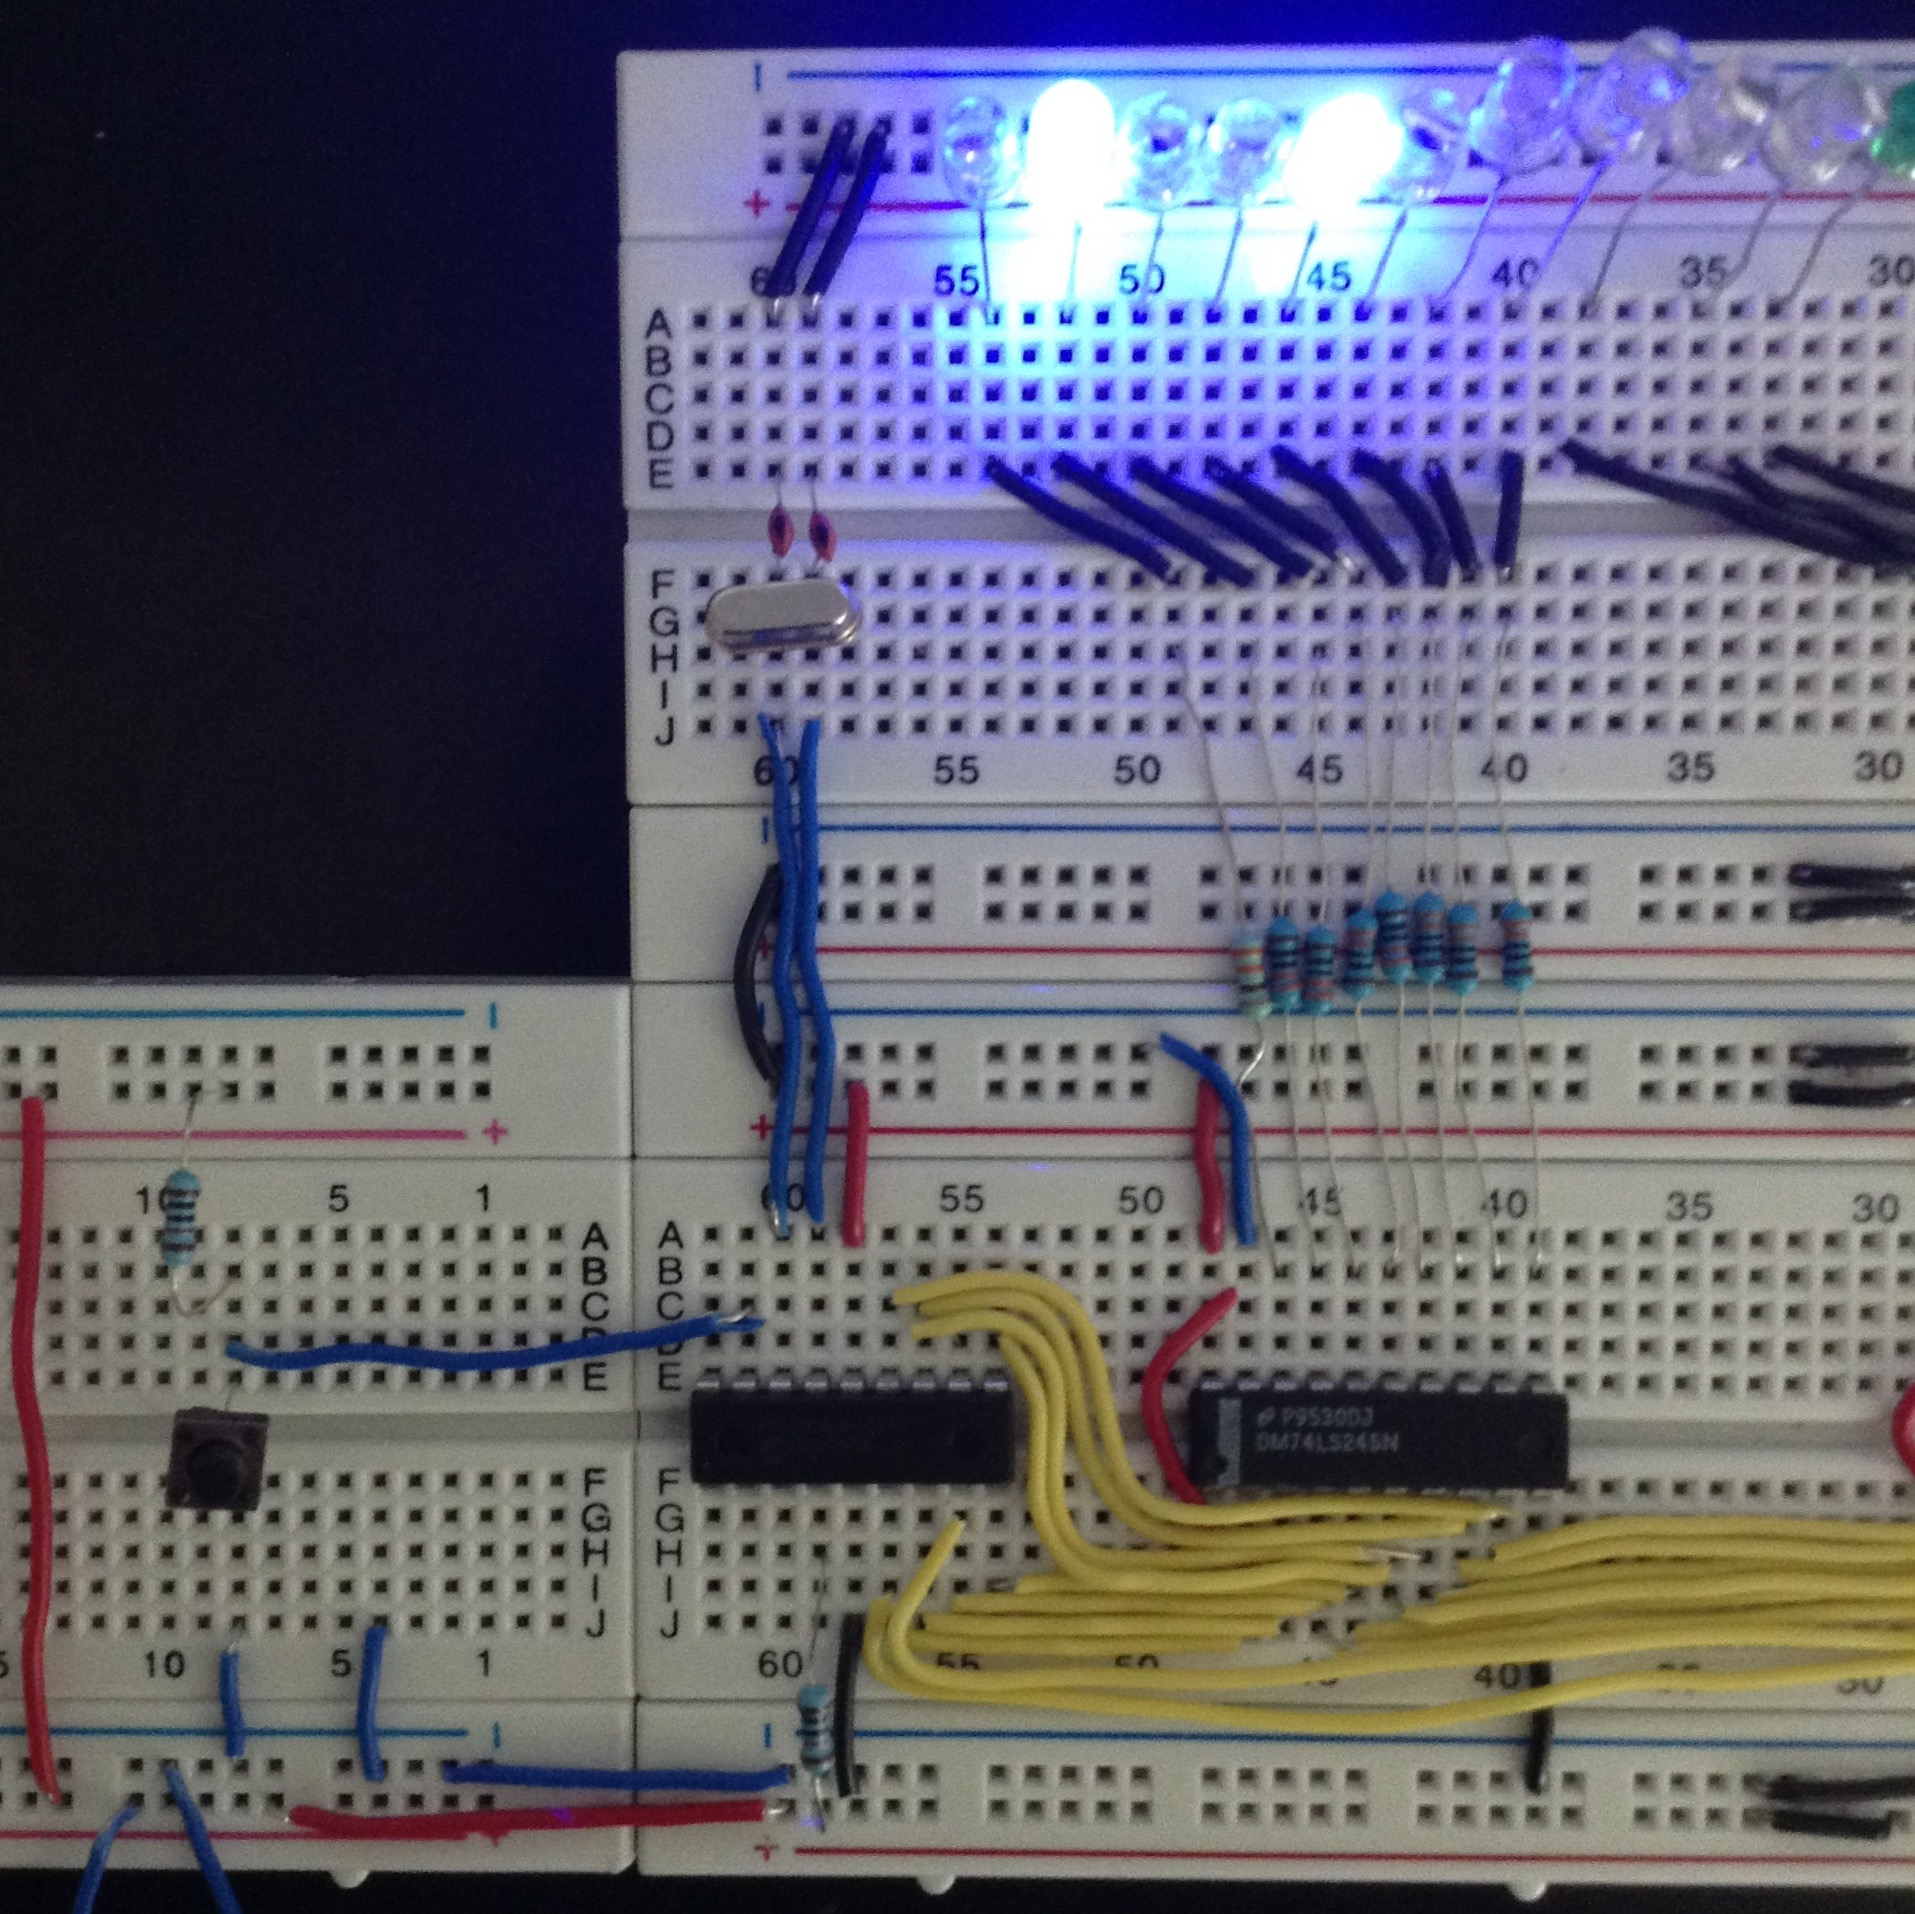
\includegraphics[width=0.45\textwidth]{cir.jpg}
  \caption{Circuito en funcionamiento.}
  \label{calentrada}
\end{figure}
 
\section{Resultados }

El conjunto de LEDs, salida del registro en aumento, mostraba un numero binario, en un rango del 1 al 255,  distinto, mayor por 1 al valor anteriormente mostrado, cada vez que un bot�n era presionado.

\section{Conclusi\'on }

Existe ruido inducido en la interacci�n con el usuario que puede causar graves problemas por lo que es necesario eliminarlo y   
para poder eliminar el ruido por medio del mismo programa por el que esta programado el micropcontrolador es necesario llamar a una rutina de un tiempo tal que deje pasar los rebotes. 


\end{document}